% Important: If latex complains about unicode characters,
% please use "\usepackage[utf8x]{inputenc}" in your preamble
% You can change the size of the picture by putting it into the construct:
% 1) \resizebox{10cm}{!}{"below picture"} to scale horizontally to 10 cm
% 2) \resizebox{!}{15cm}{"below picture"} to scale vertically to 15 cm
% 3) \resizebox{10cm}{15cm}{"below picture"} a combination of above two
% It is not recomended to use the scale option of the tikzpicture environment.
\scalebox{0.5}{
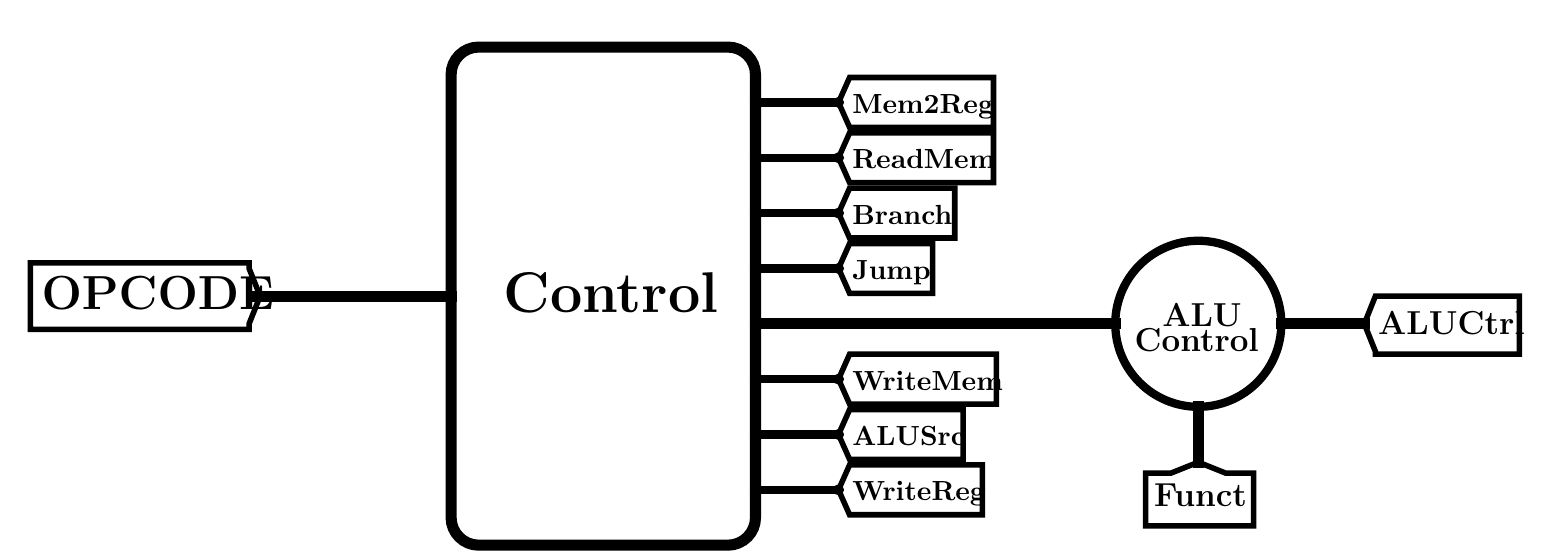
\begin{tikzpicture}[x=1pt,y=-1pt,line cap=rect]
\def\logisimfontA#1{{\fontspec{CMU Serif}#1}} % cmr equivalent
\def\logisimfontB#1{{\fontspec{CMU Bright}#1}}
\definecolor{custcol_0_0_0}{RGB}{0, 0, 0}
\definecolor{custcol_ff_ff_ff}{RGB}{255, 255, 255}
\draw [line width=4.0pt, custcol_0_0_0 ]  (422.0,137.0) -- (422.0,157.0) ;
\draw [line width=3.0pt, custcol_0_0_0 ]  (262.0,27.0) -- (292.0,27.0) ;
\draw [line width=3.0pt, custcol_0_0_0 ]  (262.0,167.0) -- (292.0,167.0) ;
\draw [line width=3.0pt, custcol_0_0_0 ]  (262.0,87.0) -- (292.0,87.0) ;
\draw [line width=3.0pt, custcol_0_0_0 ]  (262.0,147.0) -- (292.0,147.0) ;
\draw [line width=3.0pt, custcol_0_0_0 ]  (262.0,67.0) -- (292.0,67.0) ;
\draw [line width=3.0pt, custcol_0_0_0 ]  (262.0,127.0) -- (292.0,127.0) ;
\draw [line width=3.0pt, custcol_0_0_0 ]  (262.0,47.0) -- (292.0,47.0) ;
\draw [line width=4.0pt, custcol_0_0_0 ]  (452.0,107.0) -- (482.0,107.0) ;
\draw [line width=4.0pt, custcol_0_0_0 ]  (262.0,107.0) -- (392.0,107.0) ;
\draw [line width=4.0pt, custcol_0_0_0 ]  (82.0,97.0) -- (152.0,97.0) ;
\begin{pgfpicture}
   \begin{pgfmagnify}{1pt}{-1pt}
      \pgfsetrectcap
      \pgfsetcornersarced{\pgfpoint{10.0}{10.0}}
      \pgfsetlinewidth{4.0}
      \color{custcol_0_0_0}
      \pgfsetfillopacity{1.0}
      \pgfpathrectanglecorners{\pgfpoint{152.0}{7.0}}{\pgfpoint{262.0}{187.0}}
      \pgfusepath{stroke}
   \end{pgfmagnify}
\end{pgfpicture}
\logisimfontB{\fontsize{20pt}{20pt}\fontseries{bx}\selectfont\node[inner sep=0, outer sep=0, custcol_0_0_0, anchor=base west] at  (171.0,103.0)  {Control};}
\fill [line width=1.0pt, custcol_0_0_0]  (152.0,97.0) ellipse (2.0 and 2.0 );
\fill [line width=1.0pt, custcol_0_0_0]  (262.0,27.0) ellipse (2.0 and 2.0 );
\fill [line width=1.0pt, custcol_0_0_0]  (262.0,47.0) ellipse (2.0 and 2.0 );
\fill [line width=1.0pt, custcol_0_0_0]  (262.0,67.0) ellipse (2.0 and 2.0 );
\fill [line width=1.0pt, custcol_0_0_0]  (262.0,87.0) ellipse (2.0 and 2.0 );
\fill [line width=1.0pt, custcol_0_0_0]  (262.0,107.0) ellipse (2.0 and 2.0 );
\fill [line width=1.0pt, custcol_0_0_0]  (262.0,127.0) ellipse (2.0 and 2.0 );
\fill [line width=1.0pt, custcol_0_0_0]  (262.0,147.0) ellipse (2.0 and 2.0 );
\fill [line width=1.0pt, custcol_0_0_0]  (262.0,167.0) ellipse (2.0 and 2.0 );
\logisimfontB{\fontsize{10pt}{10pt}\fontseries{bx}\selectfont\node[inner sep=0, outer sep=0, custcol_0_0_0, anchor=base west] at  (297.0,151.0)  {ALUSrc};}
\draw [line width=2.0pt, custcol_0_0_0 ]  (296.0,138.0) -- (337.0,138.0) -- (337.0,156.0) -- (296.0,156.0) -- (292.0,147.0) -- cycle;
\fill [line width=2.0pt, custcol_0_0_0]  (292.0,147.0) ellipse (2.0 and 2.0 );
\logisimfontB{\fontsize{10pt}{10pt}\fontseries{bx}\selectfont\node[inner sep=0, outer sep=0, custcol_0_0_0, anchor=base west] at  (297.0,71.0)  {Branch};}
\draw [line width=2.0pt, custcol_0_0_0 ]  (296.0,58.0) -- (334.0,58.0) -- (334.0,76.0) -- (296.0,76.0) -- (292.0,67.0) -- cycle;
\fill [line width=2.0pt, custcol_0_0_0]  (292.0,67.0) ellipse (2.0 and 2.0 );
\logisimfontB{\fontsize{10pt}{10pt}\fontseries{bx}\selectfont\node[inner sep=0, outer sep=0, custcol_0_0_0, anchor=base west] at  (297.0,131.0)  {WriteMem};}
\draw [line width=2.0pt, custcol_0_0_0 ]  (296.0,118.0) -- (349.0,118.0) -- (349.0,136.0) -- (296.0,136.0) -- (292.0,127.0) -- cycle;
\fill [line width=2.0pt, custcol_0_0_0]  (292.0,127.0) ellipse (2.0 and 2.0 );
\logisimfontB{\fontsize{10pt}{10pt}\fontseries{bx}\selectfont\node[inner sep=0, outer sep=0, custcol_0_0_0, anchor=base west] at  (297.0,91.0)  {Jump};}
\draw [line width=2.0pt, custcol_0_0_0 ]  (296.0,78.0) -- (326.0,78.0) -- (326.0,96.0) -- (296.0,96.0) -- (292.0,87.0) -- cycle;
\fill [line width=2.0pt, custcol_0_0_0]  (292.0,87.0) ellipse (2.0 and 2.0 );
\logisimfontB{\fontsize{10pt}{10pt}\fontseries{bx}\selectfont\node[inner sep=0, outer sep=0, custcol_0_0_0, anchor=base west] at  (297.0,171.0)  {WriteReg};}
\draw [line width=2.0pt, custcol_0_0_0 ]  (296.0,158.0) -- (344.0,158.0) -- (344.0,176.0) -- (296.0,176.0) -- (292.0,167.0) -- cycle;
\fill [line width=2.0pt, custcol_0_0_0]  (292.0,167.0) ellipse (2.0 and 2.0 );
\logisimfontB{\fontsize{10pt}{10pt}\fontseries{bx}\selectfont\node[inner sep=0, outer sep=0, custcol_0_0_0, anchor=base west] at  (297.0,31.0)  {Mem2Reg};}
\draw [line width=2.0pt, custcol_0_0_0 ]  (296.0,18.0) -- (348.0,18.0) -- (348.0,36.0) -- (296.0,36.0) -- (292.0,27.0) -- cycle;
\fill [line width=2.0pt, custcol_0_0_0]  (292.0,27.0) ellipse (2.0 and 2.0 );
\logisimfontB{\fontsize{10pt}{10pt}\fontseries{bx}\selectfont\node[inner sep=0, outer sep=0, custcol_0_0_0, anchor=base west] at  (297.0,51.0)  {ReadMem};}
\draw [line width=2.0pt, custcol_0_0_0 ]  (296.0,38.0) -- (348.0,38.0) -- (348.0,56.0) -- (296.0,56.0) -- (292.0,47.0) -- cycle;
\fill [line width=2.0pt, custcol_0_0_0]  (292.0,47.0) ellipse (2.0 and 2.0 );
\logisimfontB{\fontsize{16pt}{16pt}\fontseries{bx}\selectfont\node[inner sep=0, outer sep=0, custcol_0_0_0, anchor=base west] at  (4.0,102.0)  {OPCODE};}
\draw [line width=2.0pt, custcol_0_0_0 ]  (0.0,85.0) -- (79.0,85.0) -- (79.0,87.0) -- (83.0,97.0) -- (79.0,107.0) -- (79.0,109.0) -- (0.0,109.0) -- cycle;
\fill [line width=2.0pt, custcol_0_0_0]  (82.0,97.0) ellipse (2.0 and 2.0 );
\draw [line width=3.0pt, custcol_0_0_0]  (422.0,107.0) ellipse (30.0 and 30.0 );
\logisimfontB{\fontsize{12pt}{12pt}\fontseries{bx}\selectfont\node[inner sep=0, outer sep=0, custcol_0_0_0, anchor=base west] at  (409.0,108.0)  {ALU};}
\logisimfontB{\fontsize{12pt}{12pt}\fontseries{bx}\selectfont\node[inner sep=0, outer sep=0, custcol_0_0_0, anchor=base west] at  (399.0,117.0)  {Control};}
\fill [line width=1.0pt, custcol_0_0_0]  (392.0,107.0) ellipse (2.0 and 2.0 );
\fill [line width=1.0pt, custcol_0_0_0]  (422.0,137.0) ellipse (2.0 and 2.0 );
\fill [line width=1.0pt, custcol_0_0_0]  (452.0,107.0) ellipse (2.0 and 2.0 );
\logisimfontB{\fontsize{12pt}{12pt}\fontseries{bx}\selectfont\node[inner sep=0, outer sep=0, custcol_0_0_0, anchor=base west] at  (406.0,173.0)  {Funct};}
\draw [line width=2.0pt, custcol_0_0_0 ]  (403.0,161.0) -- (412.0,161.0) -- (422.0,157.0) -- (432.0,161.0) -- (442.0,161.0) -- (442.0,180.0) -- (403.0,180.0) -- cycle;
\fill [line width=2.0pt, custcol_0_0_0]  (422.0,157.0) ellipse (2.0 and 2.0 );
\logisimfontB{\fontsize{12pt}{12pt}\fontseries{bx}\selectfont\node[inner sep=0, outer sep=0, custcol_0_0_0, anchor=base west] at  (487.0,111.0)  {ALUCtrl};}
\draw [line width=2.0pt, custcol_0_0_0 ]  (486.0,97.0) -- (538.0,97.0) -- (538.0,118.0) -- (486.0,118.0) -- (486.0,117.0) -- (482.0,107.0) -- cycle;
\fill [line width=2.0pt, custcol_0_0_0]  (482.0,107.0) ellipse (2.0 and 2.0 );
\end{tikzpicture}
}